\documentclass[a4paper, 12pt]{report}
\usepackage{graphicx}
\usepackage[french]{babel}
\usepackage[utf8]{inputenc}
\usepackage[T1]{fontenc}
\usepackage{multirow}
\usepackage{listings}
\usepackage{float}
\usepackage[french]{babel}
\usepackage[breaklinks]{hyperref}
\hypersetup{pageanchor=false}

\begin{document}

\begin{titlepage}
  \begin{center}
    \begin{tabular*}{\textwidth}{l@{\extracolsep{\fill}}r}
      
\includegraphics[height=1.5cm]{images/m1info.png}      
    \end{tabular*}
    \small 
    \rule{\textwidth}{.5pt}~\\
    \large 
    \textsc{Université Paris 8 - Vincennes à Saint-Denis}\vspace{0.5cm}\\
    \textbf{Master Informatique des Systèmes Embarqués}\vspace{3.0cm}\\
    \Large
    \textbf{Rapport de projet tuteuré}\vspace{1.5cm}\\
    \large
    \textbf{Samuel \textsc{de Vals}}\\
		\textbf{Paul \textsc{Vialart}}\vspace{1.5cm}\\
    Date de soutenance : le 19/01/2017\vspace{1.75cm}\\
  \end{center}\vspace{1.5cm}~\\
  \begin{tabular}{ll}
    \hspace{-0.45cm}Tuteur -- Université~:~&~Sylvia \textsc{Chalençon}
  \end{tabular}
\end{titlepage}

\newpage\null\newpage

\chapter*{Résumé}
\markboth{\sc Résumé}{}
\addcontentsline{toc}{chapter}{Résumé} 
TODO: Résumé du projet et des tâches accomplies

\chapter*{Introduction}
\markboth{\sc Introduction}{}
\addcontentsline{toc}{chapter}{Introduction}
\input{teX/001_introduction.tex}

%adding content into the summary page /!\ need 2 compilations
\addcontentsline{toc}{chapter}{Le choix de l'API three.JS}
\addcontentsline{toc}{chapter}{Le bruit de Perlin}

\tableofcontents

\chapter*{Le choix de l'API three.JS}
\markboth{\sc Le choix de l'API three.JS}{}
Nous avons tout d'abord découpé le projet en différentes tâches à réaliser afin de le mener à son terme. Voici un schéma représentant les principales étapes d'élaboration du projet.

\begin{center}
	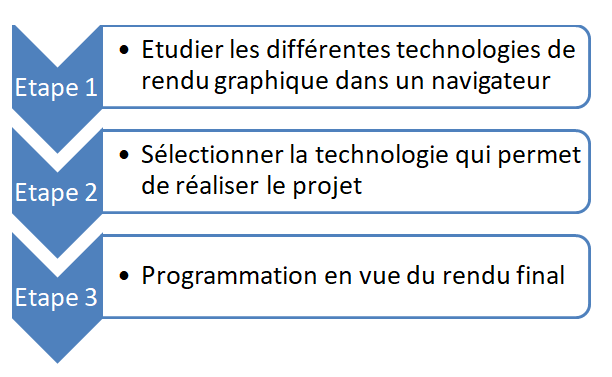
\includegraphics[height=7cm]{images/Processus_DEV.png}\\
	\textit{Processus de développement utilisé au cours du projet}\\
\end{center}

\newpage
Pour ce projet, nous avons choisi l'API three.JS. Celle-ci permet de faire du WebGL de façon simple et facilite la mise en œuvre du projet. En effet, ce projet est notre premier contact avec le domaine du WebGL. Avec sa communauté active, ses nombreux tutoriels et ses exemples détaillés, three.JS semble être la méthode la plus simple pour modéliser l'environnement qui nous a été demandé.

Cette API permet de simuler une vaste variété de rendus en 3D paramétrables. Il peut s'agir de décors, de personnages, d'effets de particules, etc.

\begin{center}
	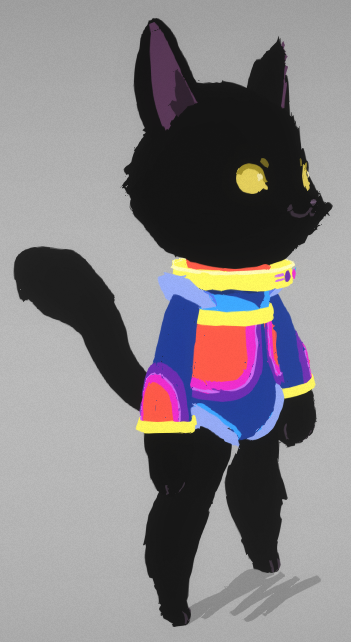
\includegraphics[height=6cm]{images/threeJS_poly_cat.png}\\
	\textit{Exemple de personnage 3D généré avec le module Poly de three.JS}
\end{center}

\begin{center}
	
\includegraphics[height=6cm]{images/threeJS_poly_particle.png}\\
	\textit{three.JS permet également de reproduire des effets de particules avancés...}
\end{center}

\begin{center}
	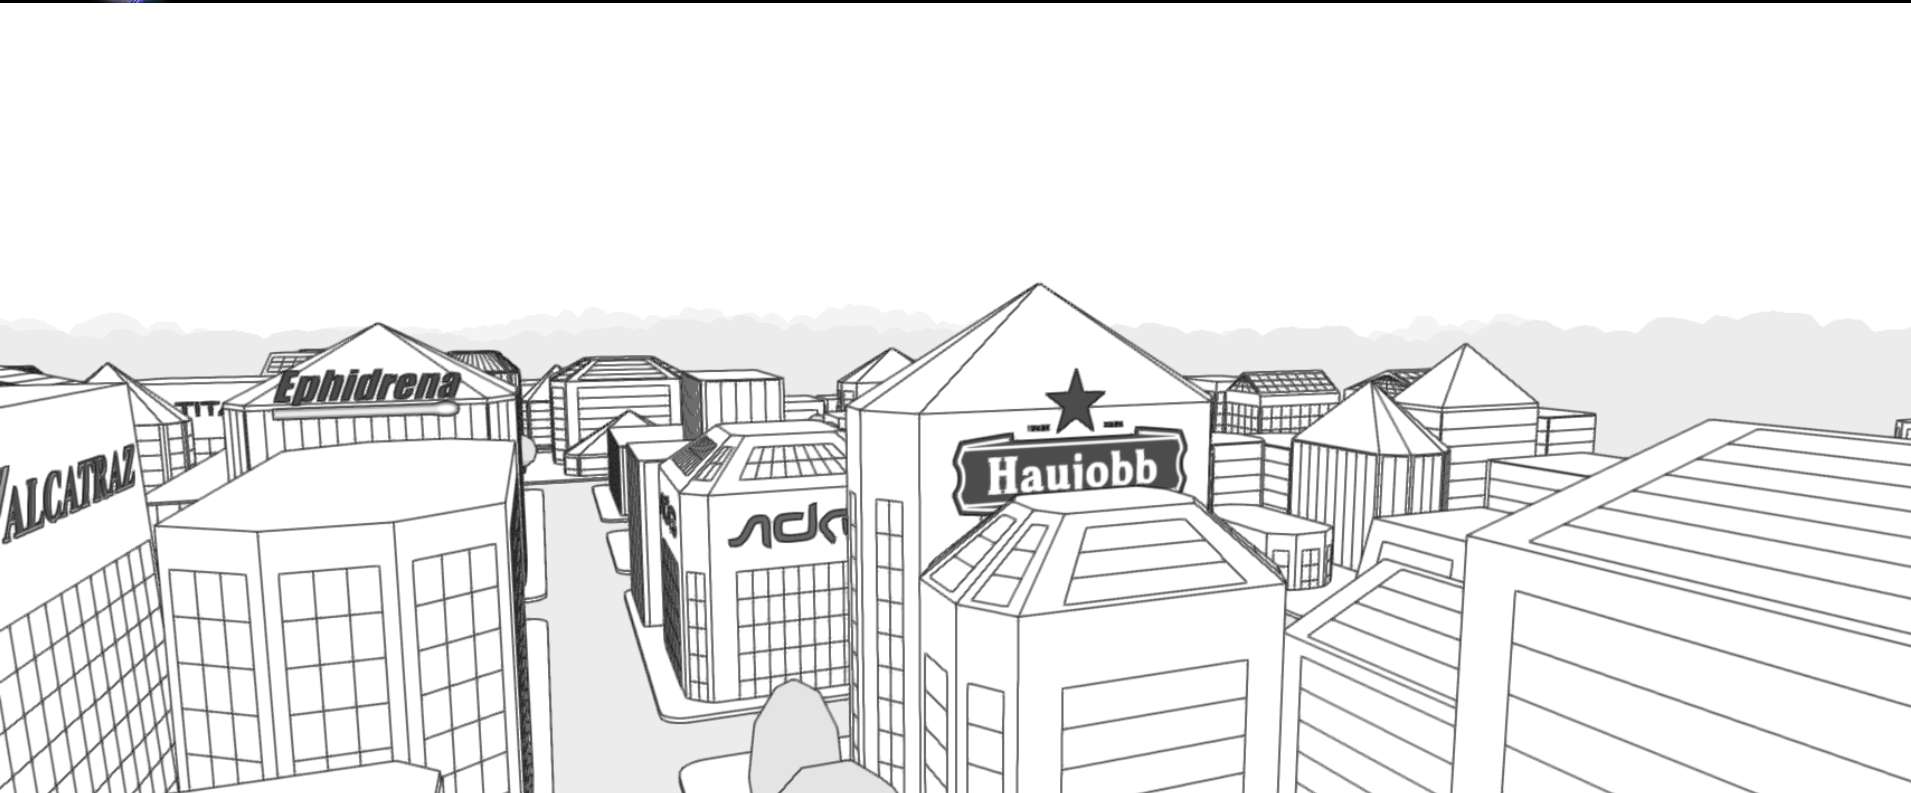
\includegraphics[height=6cm]{images/threeJS_poly_city.png}\\
	\textit{... voire des villes entières.}
\end{center}



Dans notre cas, la page web génère un monde virtuel avec le bruit de Perlin. Afin de partir sur une modélisation cubique, proche du rendu final en style Lego, nous nous sommes orientés vers une déclinaison de l'API reproduisant l'univers du jeu vidéo Minecraft, réputé pour son univers tout en cubes. Voici le rendu graphique de l'exemple :

\begin{center}
	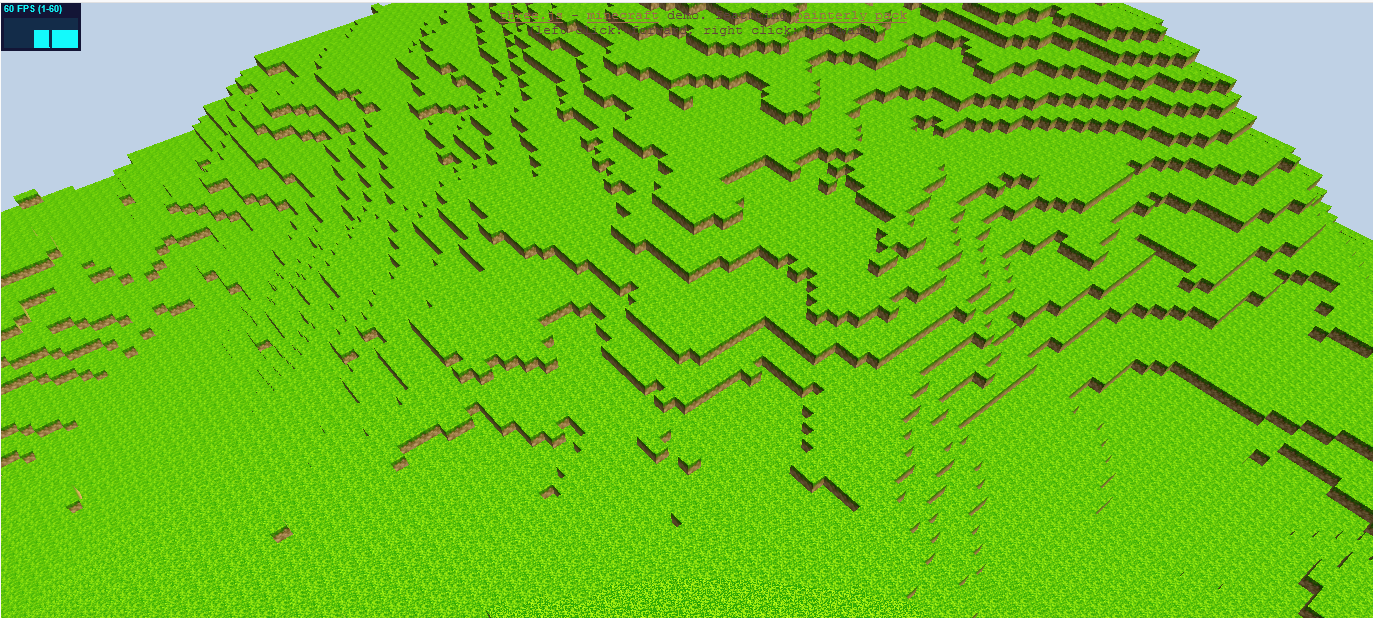
\includegraphics[height=6cm]{images/threeJS_minecraft.png}\\
	\textit{Exemple du monde virtuel généré avec l'API three.JS}
	\footnote{Le code source de l'exemple de l'API three.JS se trouve là : \url{https://github.com/mrdoob/three.js/blob/master/examples/webgl_geometry_minecraft.html}}
\end{center}

Il a ensuite fallu adapter le projet afin de mettre le code source HTML, CSS, et JS dans des fichiers séparés.

\begin{center}
	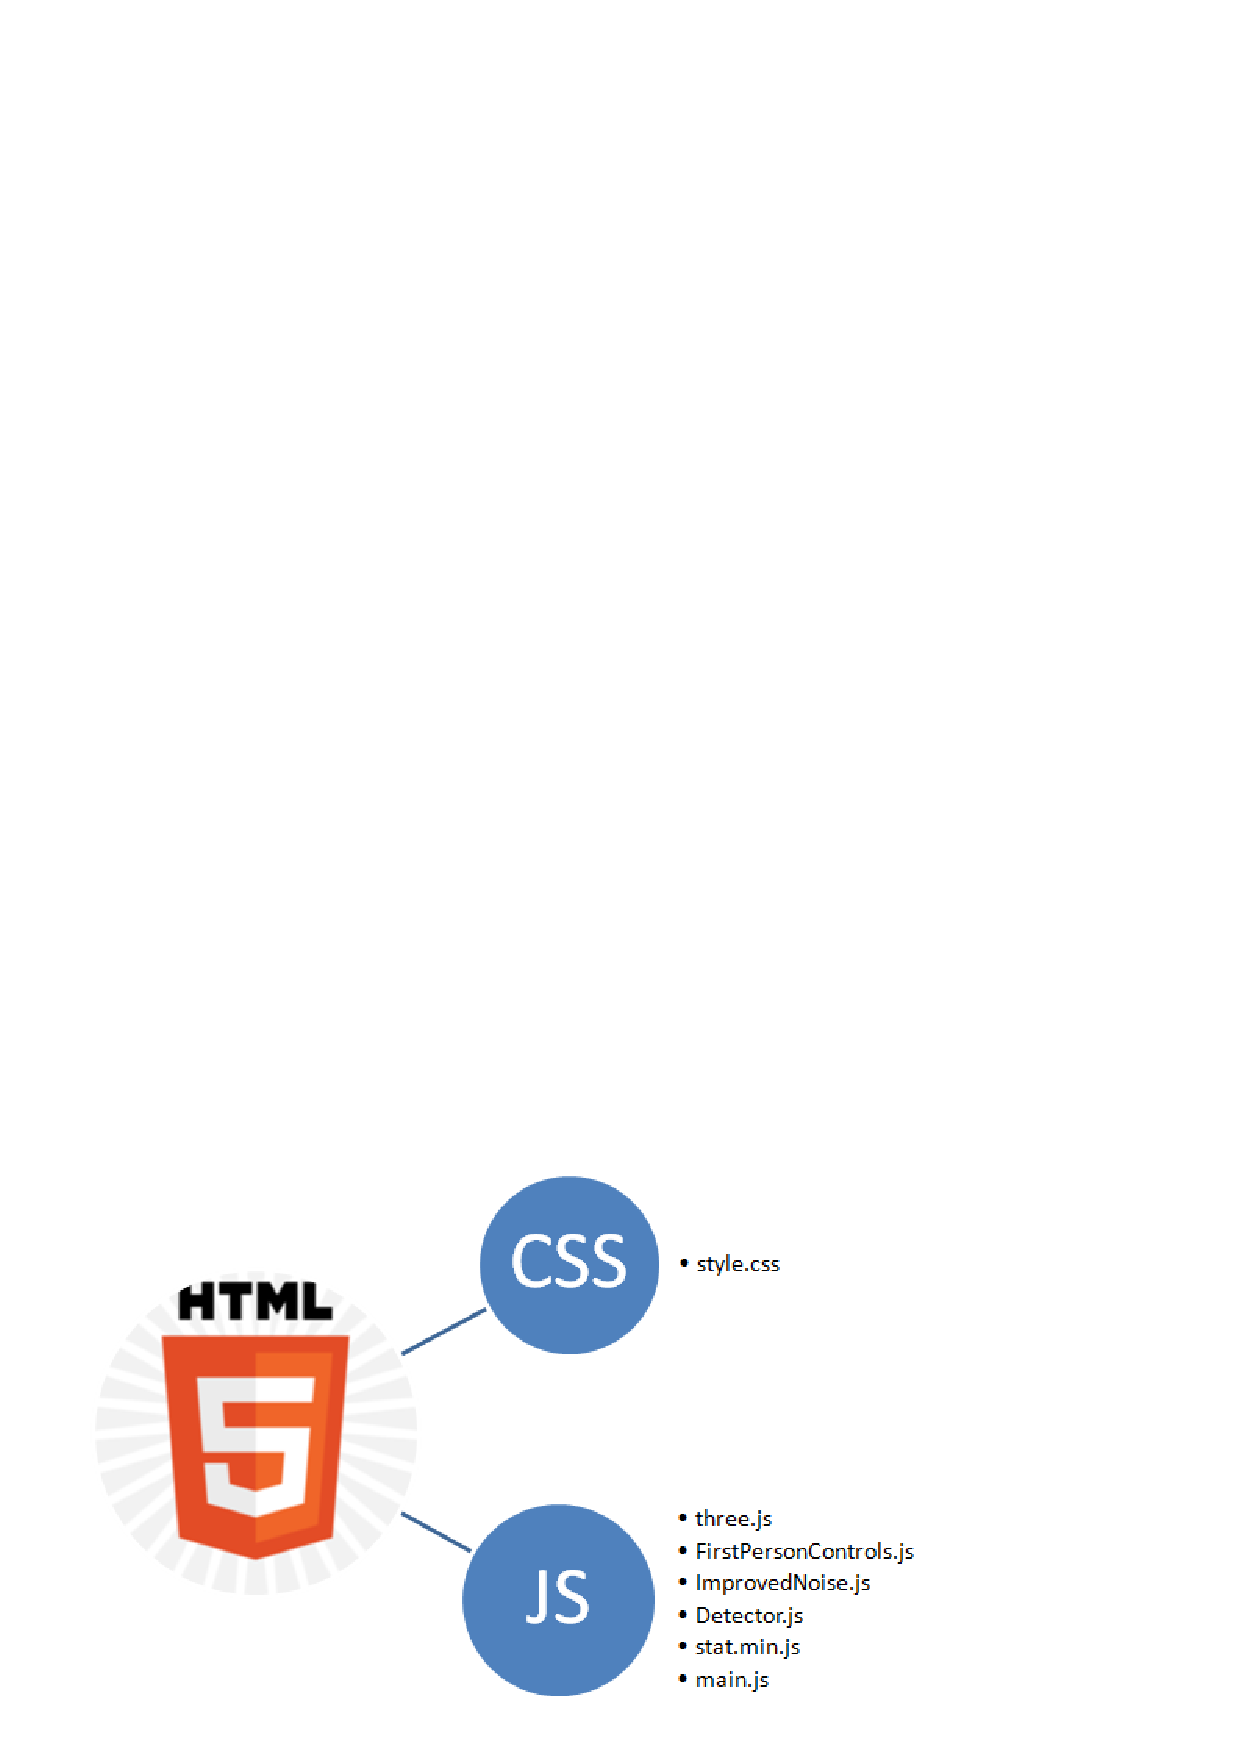
\includegraphics[height=6cm]{images/ProFileOrganisation.png}\\
	\textit{Structure du projet}
\end{center}

\chapter*{Le bruit de Perlin}
\markboth{\sc Le bruit de Perlin}{}
Le bruit de Perlin est très utilisé dans la génération d'image. Effet, ce bruit permet de déterminer une élévation d'un sommet de N-dimension (dans notre cas 3). Nous avons donc implémenté un algorithme de afin de générer. L'algorithme se divise en deux temps :

\begin{enumerate}
	\item Initialisation
	\item Calcul
\end{enumerate}

La phase d'initialisation consite à avoir un tableau de 512 éléments bien mélangés compris entre 0 et 255. Enfin, le tableau se répète à partir de la valeur 256 (tab[0] = tab[256], et ainsi de suite). La phase de calcul est plus compliquée, car elle se découpe en plusieurs étapes. Le principe de l'algorithme est de retourner une même valeur en fonction d'un x, d'un y, et d'un z donné. On place x, y , z dans l'interval [0;255] avec un "et" logique. Ensuite on calcul les coordonnées en gradient du cube dans l'espace. Enfin, on calcul la valeur de retour. Ken Perlin a ensuite amélioré cet algorithme, afin qu'il soit plus performant en terme de calcul et de résultat. Cette version s'appelle le bruit de simplex.

Afin de générer aléatoirement un monde virtuel, il est necessaire de remplir le tableau aléatoirement à chaque démarrage du projet. En effet, sinon on obtiendra toujours la même monde carte, car le tableau de permutation reste toujours le même entre deux chargements.



\end{document}